%%%%%%%%%%%%%%%%%%%%%%%%%%%%%%%%%%%%%%%%%%%%%%%%%%%%%%%%%%%%%%%%%%%%%%%%%%%%%%%%
% Narrative CV — Dr. Dipankar Bhattacharya
% Fellowship / grant applications | general scientific audience
% Compiled: narrative-cv.pdf  |  Companion: narrative-cv.html
%%%%%%%%%%%%%%%%%%%%%%%%%%%%%%%%%%%%%%%%%%%%%%%%%%%%%%%%%%%%%%%%%%%%%%%%%%%%%%%%
\documentclass[11pt,a4paper]{article}

\usepackage[T1]{fontenc}
\usepackage[utf8]{inputenc}
\usepackage[p,osf,swashQ]{cochineal}
\usepackage[medium,bold]{cabin}
\usepackage[english]{babel}
\usepackage[a4paper,margin=2.0cm,top=2.0cm,bottom=2.0cm]{geometry}
\usepackage{xcolor}
\usepackage{booktabs}
\usepackage{enumitem}
\usepackage{titlesec}
\usepackage{hyperref}

\definecolor{accent}{HTML}{1B365D}
\definecolor{charcoal}{HTML}{444444}
% TikZ figures for narrative-cv.tex (load after accent/charcoal colours are defined)
\usepackage{tikz}
\usetikzlibrary{positioning, arrows.meta, calc, shapes.geometric}

\definecolor{health}{HTML}{2E86AB}
\definecolor{cable}{HTML}{A23B72}
\definecolor{manuf}{HTML}{F18F01}
\definecolor{rehab}{HTML}{C73E1D}
\definecolor{metricbg}{HTML}{F4F6F9}

\newcommand{\NarrativeMetricsFigure}{%
\begin{center}
\renewcommand{\arraystretch}{1.25}
\begin{tabular}{@{}cccc@{}}
  \fcolorbox{accent!30}{metricbg}{\begin{tabular}{c}\textbf{\large 9}\\Journal articles\\\scriptsize 8 published, 1 accepted\end{tabular}} &
  \fcolorbox{accent!30}{metricbg}{\begin{tabular}{c}\textbf{\large 4}\\Conference papers\\\scriptsize incl.\ IROS 2026 accepted\end{tabular}} &
  \fcolorbox{accent!30}{metricbg}{\begin{tabular}{c}\textbf{\large 1}\\Book chapter\\\scriptsize Springer, 2019\end{tabular}} &
  \fcolorbox{accent!30}{metricbg}{\begin{tabular}{c}\textbf{\large 6}\\Countries\\\scriptsize IN, NZ, HK, CN, FR, UK\end{tabular}} \\[6pt]
  \fcolorbox{accent!30}{metricbg}{\begin{tabular}{c}\textbf{\large 5}\\Grants\\\scriptsize 2 led; 2 co-authored\end{tabular}} &
  \fcolorbox{accent!30}{metricbg}{\begin{tabular}{c}\textbf{\large 6+}\\Students supervised\\\scriptsize 2 MEng; 3 PhD; 1 placement\end{tabular}} &
  \fcolorbox{accent!30}{metricbg}{\begin{tabular}{c}\textbf{\large EUR 276k}\\MSCA fellowship\\\scriptsize 24-month independent PI\end{tabular}} &
  \fcolorbox{accent!30}{metricbg}{\begin{tabular}{c}\textbf{\large 10+}\\Invited talks\\\scriptsize Imperial, WRC, ICMA, ETA\end{tabular}}
\end{tabular}
\end{center}}

\newcommand{\NarrativeTimelineFigure}{%
\begin{center}
\small
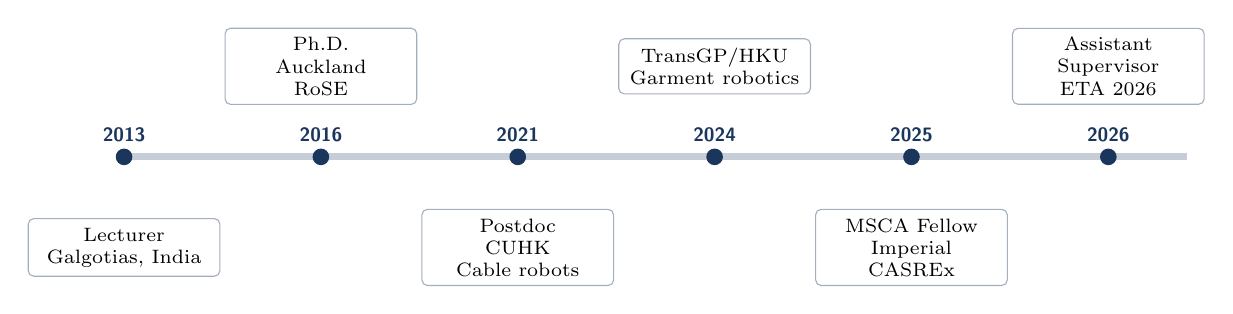
\begin{tikzpicture}[
  phase/.style={rectangle, rounded corners=2pt, draw=accent!40, fill=white, align=center, font=\scriptsize, text width=2.2cm}
]
  \draw[accent!25, line width=2.5pt] (0,0) -- (13.5,0);
  \foreach \x/\yr/\pos/\txt in {
    0/2013/below/{Lecturer\\Galgotias, India},
    2.5/2016/above/{Ph.D.\\Auckland\\RoSE},
    5.0/2021/below/{Postdoc\\CUHK\\Cable robots},
    7.5/2024/above/{TransGP/HKU\\Garment robotics},
    10.0/2025/below/{MSCA Fellow\\Imperial\\CASREx},
    12.5/2026/above/{Assistant\\Supervisor\\ETA 2026}
  }{
    \fill[accent] (\x,0) circle (3pt);
    \node[font=\scriptsize\bfseries\sffamily, text=accent, yshift=8pt] at (\x,0) {\yr};
    \ifnum\pdfstrcmp{\pos}{below}=0
      \node[phase] at (\x,-1.15) {\txt};
    \else
      \node[phase] at (\x,1.15) {\txt};
    \fi
  }
\end{tikzpicture}
\end{center}}

\newcommand{\NarrativeDomainsFigure}{%
\begin{center}
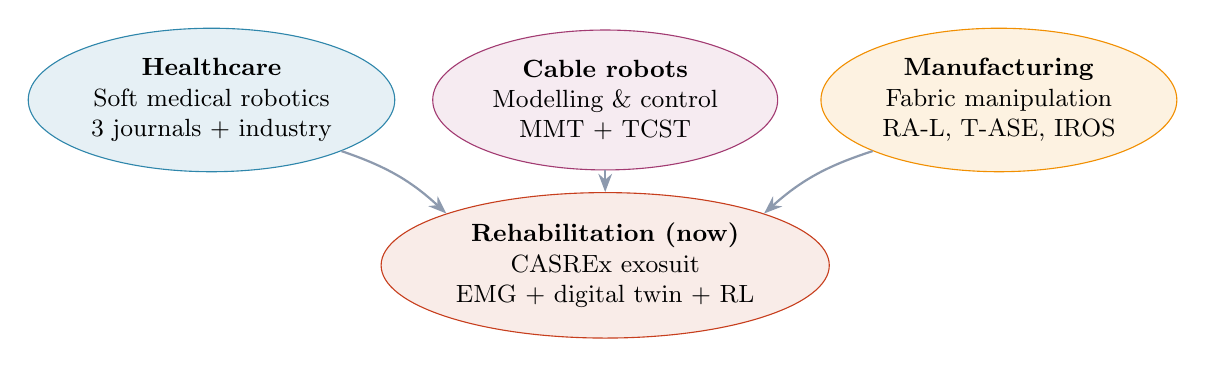
\begin{tikzpicture}
  \node[ellipse, draw=health, fill=health!12, minimum width=3.4cm, minimum height=1.4cm, align=center, font=\small] (h) at (0,0) {\textbf{Healthcare}\\Soft medical robotics\\3 journals + industry};
  \node[ellipse, draw=cable, fill=cable!10, minimum width=3.4cm, minimum height=1.4cm, align=center, font=\small] (c) at (5.0,0) {\textbf{Cable robots}\\Modelling \& control\\MMT + TCST};
  \node[ellipse, draw=manuf, fill=manuf!12, minimum width=3.4cm, minimum height=1.4cm, align=center, font=\small] (m) at (10.0,0) {\textbf{Manufacturing}\\Fabric manipulation\\RA-L, T-ASE, IROS};
  \node[ellipse, draw=rehab, fill=rehab!10, minimum width=3.6cm, minimum height=1.4cm, align=center, font=\small] (r) at (5.0,-2.1) {\textbf{Rehabilitation (now)}\\CASREx exosuit\\EMG + digital twin + RL};
  \draw[-{Stealth}, accent!50, thick] (h.south east) to[bend left=12] (r.north west);
  \draw[-{Stealth}, accent!50, thick] (c.south) -- (r.north);
  \draw[-{Stealth}, accent!50, thick] (m.south west) to[bend right=12] (r.north east);
\end{tikzpicture}
\end{center}}


\hypersetup{colorlinks=true,allcolors=accent,breaklinks=true}
\setlength{\parindent}{0pt}
\setlength{\parskip}{0.45em}

\titleformat{\section}{\Large\bfseries\sffamily\color{accent}}{}{0pt}{}[\vspace{-0.2em}\rule{\linewidth}{0.8pt}]
\titleformat{\subsection}{\large\bfseries\sffamily\color{accent}}{}{0pt}{}
\titlespacing*{\section}{0pt}{0.9em}{0.35em}
\titlespacing*{\subsection}{0pt}{0.7em}{0.25em}

\newcommand{\btit}[1]{\textbf{\textit{#1}}}
\newcommand{\guidebox}[2]{%
  \par\small\noindent\fcolorbox{accent!40}{metricbg}{%
    \begin{minipage}{0.97\linewidth}\vspace{0.25em}
    \textbf{\sffamily #1}\\[0.2em]#2\vspace{0.25em}
    \end{minipage}}}

\begin{document}

% ============================================================================
\thispagestyle{empty}
\begin{center}
  {\Huge\bfseries\sffamily\color{accent} Narrative CV}\\[0.3em]
  {\large\bfseries Dr. Dipankar Bhattacharya, Ph.D.}\\[0.15em]
  {\normalsize Marie Sk\l{}odowska-Curie Postdoctoral Fellow}\\[0.08em]
  {\normalsize Dyson School of Design Engineering, Imperial College London}\\[0.12em]
  {\small \href{mailto:d.bhattacharya1@imperial.ac.uk}{d.bhattacharya1@imperial.ac.uk}
  \textbar{} \href{https://profiles.imperial.ac.uk/d.bhattacharya1/about}{Imperial Profile}
  \textbar{} \href{https://bhattner143.github.io/dips/narrative-cv.html}{Interactive version}}
\end{center}

\section*{How to use this document}

This file contains \textbf{two narrative CV versions} plus \textbf{visual summaries}. Narrative CVs are prose-based accounts of achievement---not lists---used by UKRI, Horizon Europe, fellowships, and promotion panels.

\begin{center}
\renewcommand{\arraystretch}{1.35}
\begin{tabular}{@{}p{2.4cm}p{4.8cm}p{4.8cm}p{3.2cm}@{}}
\toprule
\textbf{\sffamily Version} & \textbf{\sffamily What it is} & \textbf{\sffamily When to use} & \textbf{\sffamily Typical limit} \\
\midrule
\textbf{Short} (see p.\,4) &
Concise overview: identity, CASREx, career arc, impact in $\sim$370 words. &
Form word boxes; MSCA summaries; cover letters; reviewer first pass; LinkedIn / website bio. &
300--400 words \\
\addlinespace
\textbf{Long} (see p.\,3) &
Full narrative with quantified evidence, contextualised outputs, collaboration, teaching, and future direction. &
UKRI narrative CV modules; fellowship applications; promotion dossiers; European Talent Academy; interview preparation. &
400--800 words per module (check funder) \\
\addlinespace
\textbf{Figures} (pp.\,2--3) &
Metrics dashboard, career timeline, research-domain map. &
Paste into PDF applications; present in seminars; use \texttt{narrative-cv.html} for interactive viewing. &
Visual supplement \\
\bottomrule
\end{tabular}
\end{center}

\guidebox{Tip from narrative-CV training (Ines)}{%
Narrative CVs benefit from \textbf{visualisation}: a metrics snapshot and career map help reviewers grasp breadth quickly before reading prose. Use the figures on the following pages alongside either the short or long text.}

\newpage

% ============================================================================
\section*{Research impact at a glance}
\NarrativeMetricsFigure

\vspace{0.3em}
\noindent\small\sffamily Quantified from \texttt{own-bib.bib}, \texttt{cv-simple.pdf}, and \texttt{Profile.pdf} (March 2026). Journal count: 8 published + 1 accepted (IEEE T-ASE). Conference count: 3 published + 1 accepted (IROS 2026). Grants: MSCA (EUR~276,187.92, lead), BvW (NZD~39,000, lead), 2 ITF co-authored, 1 travel grant.

\section*{Career timeline}
\NarrativeTimelineFigure

\section*{Research domains and how they connect}
\NarrativeDomainsFigure

\newpage
\label{page:long}

% ============================================================================
\section*{Long narrative CV}

\subsection*{Research identity and expertise}
My distinctive contribution sits at the crossover of \textbf{soft and cable-driven robotics}, \textbf{human-centred control}, and \textbf{learning-enabled systems} for healthcare, rehabilitation, and manufacturing. Across \textbf{9 journal articles} (8 published, 1 accepted), \textbf{4 conference papers}, and \textbf{1 Springer book chapter}, I have built a coherent line of work: model deformable systems, estimate state under uncertainty, and close the loop with adaptive control and learning.

I am Marie Sk\l{}odowska-Curie Postdoctoral Fellow at Imperial College London, where I lead \btit{CASREx}---a \textbf{24-month, EUR~276,187.92} Horizon Europe fellowship (Grant No.~101205678) and the most independent stage of my career.

\subsection*{Current fellowship}
After stroke, many people can reach but cannot keep the arm stable when bumped or loaded. The UK RATULS trial (n=770) showed conventional robot therapy did not consistently beat usual care. CASREx develops a soft, cable-driven upper-arm exosuit that targets this \emph{stability} problem---not only movement---using human experiments, muscle recordings (EMG), a digital twin, and machine learning. The project extends my prior soft-robotics and control work into rehabilitation with direct societal relevance.

At Imperial's Morph Lab, I also supervise \textbf{2 MEng placement students}, teach robotics simulation (DESE71002), deliver seminars, run Morph Lab training, and pursue \textbf{2 Imperial Connect Fund} collaborations. I was selected for the \textbf{European Talent Academy 2026} (Imperial, TU Munich, Politecnico di Milano).

\subsection*{Career development with contextualised outputs}
\textbf{Ph.D., Auckland (2016--2021):} Built RoSE, a robotic soft esophagus for stent testing; \textbf{3 journal articles}, \textbf{2 conference papers}, \textbf{1 book chapter}. Industry contract with BvW Holding (\textbf{NZD~39,000}) led to \textit{Soft Robotics} (2021) and \textit{IEEE TIE} (2021)---my first translation from lab to external partner.

\textbf{Postdoc, CUHK (2021--2024):} Cable-robot modelling and control; first-author \textit{Mechanism and Machine Theory} (2025) and \textit{IEEE TCST} (2023); co-authored \textbf{2 ITF grant proposals}; mentored UG, placement, and PhD students; visiting fellowship at LS2N, Nantes.

\textbf{TransGP / HKU (2024--2025):} Led garment-robotics programme; built industrial fabric testbeds; outputs include \textit{IEEE RA-L} (2025), \textit{IEEE T-ASE} (2026, accepted), \textit{IEEE IROS} (2026, accepted), and \textit{IEEE ICMA} (2025)---demonstrating team leadership, hardware delivery, and publication in parallel.

\subsection*{Doctoral contribution: RoSE (\textit{Soft Robotics}, 2021)}
Endoprosthetic stent migration and swallow dysfunction are difficult to study reproducibly in patients. During my Ph.D.\ at Auckland, I co-developed \btit{RoSE}, a pneumatic soft-robotic esophagus for controlled in vitro testing of covered self-expandable metal stents. As first author, I contributed to the layered actuator design and fabrication workflow, programmed symmetric and peristaltic actuation protocols, and experimentally validated stent radial force, migration displacement, and intrabolus pressure signatures under manometry---including industry-funded testing (BvW Holding, NZD~39,000). Published in \textit{Soft Robotics} (2021), RoSE established an early benchtop approach to physiologically structured stent evaluation. Its continuing relevance is reflected in subsequent biomimetic esophageal motility research (\textit{Nature Communications}, 2026), which cites RoSE and references its circumferential pneumatic design while advancing independent longitudinal--circumferential actuation and biohybrid tissue modelling.

\subsection*{Impact, collaboration, and community}
\textbf{Impact:} Medical-device testing (BvW); garment-manufacturing automation (TransGP); upper-limb rehabilitation (CASREx). \textbf{Collaboration:} \textbf{6 countries} (India, New Zealand, Hong Kong, China, France, UK); industry and academic partners; MSCA and ETA networks. \textbf{Community:} Reviewer for \textit{IEEE RA-L}, \textit{ICRA}, \textit{ASME JMR}; \textbf{10+ invited talks} including World Robotics Conference 2025 and IEEE ICMA 2025 workshop; supervision of \textbf{6+ students} (2 MEng, 3 PhD at HKU, 1 placement at CUHK).

\subsection*{Recognition and future promise}
MSCA fellowship; European Talent Academy 2026; Best Conference Paper, RiTA 2017; GATE 99.12\% (2011); Marie Curie Alumni Association. Near-term: validate CASREx as an impedance-aware rehabilitation framework. Medium-term: establish a research programme on human-centred soft and cable-driven robots across healthcare and manufacturing.

\newpage
\label{page:short}

% ============================================================================
\section*{Short narrative CV (370 words)}

I am a robotics researcher developing intelligent machines for healthcare, rehabilitation, and manufacturing---with \textbf{9 journal articles}, \textbf{4 conference papers}, and research across \textbf{6 countries}. My work addresses settings where the body or handled material is soft, deformable, and easily disturbed.

I lead \btit{CASREx}, a Marie Sk\l{}odowska-Curie Horizon Europe fellowship at Imperial College London (\textbf{EUR~276,187.92}; 24 months; Grant No.~101205678) on a cable-driven soft exosuit for upper-arm muscle-impairment rehabilitation. Everyday stability---carrying a cup without spilling when bumped---depends on how the brain adjusts arm stiffness. After stroke, this is often impaired. CASREx combines human experiments, muscle-signal recordings, a digital twin, and machine learning to translate healthy stiffness strategies into adaptive patient assistance.

My career has moved deliberately: Ph.D.\ at Auckland (RoSE soft esophagus; \textbf{NZD~39,000} industry funding; \textit{Soft Robotics} and \textit{IEEE TIE}); postdoc at CUHK (cable-robot modelling; \textit{MMT} 2025, \textit{IEEE TCST} 2023); Senior Research Engineer at TransGP (led fabric-robotics programme; \textit{IEEE RA-L} 2025, \textit{T-ASE} 2026 accepted, \textit{IROS} 2026 accepted). I now supervise \textbf{2 MEng students} at Imperial, mentor doctoral researchers at HKU, review for major robotics venues, and was selected for the \textbf{European Talent Academy 2026}.

My aim is a long-term programme on human-centred soft robotics---helping people recover stability, and building automation that works with the real world.

\vspace{0.5em}
\begin{center}
\small\color{charcoal}
Sources: \texttt{cv-simple.pdf}, \texttt{Profile.pdf}, \texttt{own-bib.bib}.
Interactive figures: \href{https://bhattner143.github.io/dips/narrative-cv.html}{narrative-cv.html}
\end{center}

\end{document}
